\iffalse
                       
                        
                        
                        
                    
                        \author{AI24BTECH11006 - Bugada Roopansha}
                        \section{ME}
                        \chapter{2015}
                        \fi
 
    \item A machine element is subjected to the following bi-axial state of stress: $\sigma_1 = 80$ MPa; $\sigma_2 = 20$ MPa; $T_{xy} = 40$ MPa. If the shear strength of the material is $100$ MPa, the factor of safety as per Tresca's maximum shear stress theory is
    \begin{enumerate}
        \item $1.0$
        \item $2.0$
        \item $2.5$
        \item $3.3$
    \end{enumerate} 


    \item A cantilever beam with flexural rigidity of $200$ Nm is loaded as shown in the figure. The deflection \brak{\text{in mm}} at the tip of the beam is $\cdots$

\begin{center}
    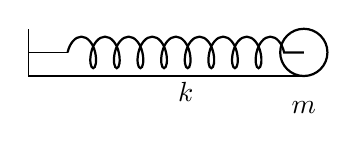
\begin{tikzpicture}
        % Drawing the spring
        \draw[thick, decoration={coil,aspect=0.5,segment length=3mm, amplitude=2mm}, decorate] (0,0) -- (3,0);
        \node at (1.5,-0.5) {$k$};

        % Drawing the disc
        \draw[thick] (3,0) circle (0.3);
        \node at (3,-0.7) {$m$};

        \draw (-0.5,-0.3) -- (3,-0.3);
        \draw (-0.5,0) -- (0,0);
        \draw (-0.5,-0.3) -- (-0.5,0.3);
    \end{tikzpicture}
    \end{center}



 \item A precision instrument package $\brak{m = 1 \text{kg}}$ needs to be mounted on a surface vibrating at $60$ Hz. It is desired that only $5\%$ of the base surface vibration amplitude be transmitted to the instrument. Assume that the isolation is designed with its natural frequency significantly lesser than $60$ Hz, so that the effect of damping may be ignored. The stiffness $\brak{\text{in}\frac{N}{m}}$ of the required mounting pad is$\cdots$

\item A horizontal plate has been joined to a vertical post using four rivets arranged as shown in the figure. The magnitude of the load on the worst-loaded rivet \brak{\text{in N}} is $\cdots$

\begin{center}
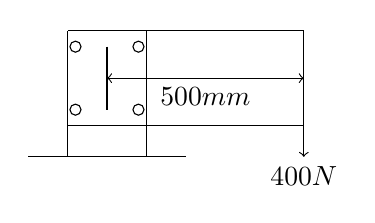
\begin{tikzpicture}
    % Draw rivets as circles
    \draw (0.4, 0.4) circle (2pt) node[above right] {};
    \draw (0.4, -0.4) circle (2pt) node[below right] {};
    \draw (-0.4, 0.4) circle (2pt) node[above left] {};
    \draw (-0.4, -0.4) circle (2pt) node[below left] {};

    

    % Draw horizontal and vertical distances between rivets
    \draw (0.5, 0.6) -- (-0.5, 0.6) ;
    \draw (0.5, -0.6) -- (-0.5, -0.6);
    \draw (-0.5, -0.6) -- (-0.5,0.6);
    \draw (0.5, -0.6) -- (0.5, 0.6);
    \draw (0.5, -0.6) -- (0.5, -1);
    \draw (-0.5, -0.6) -- (-0.5, -1);
   \draw (1, -1) -- (-1, -1);
    \draw (0.5, 0.6) -- (2.5, 0.6) ;
    \draw (0.5, -0.6) -- (2.5, -0.6) ;
    \draw (2.5 ,0.6) -- (2.5 ,-0.6);
    \draw[->] (2.5,-0.6) -- (2.5 ,-1) node[below]{$400N$} ;
    \draw (0,0.4) -- (0,-0.4);
    \draw[<->] (0,0) -- (2.5,0) node[below,midway]{$500 mm$};
\end{tikzpicture}
\end{center}


 \item For flow through a pipe of radius $R$, the velocity and temperature distribution are as follows:
    $u\brak{r, x} = C_1$, and $T\brak{r, x} = C_2 \sbrak{1 - \brak{\frac{r}{R}}^2}$, where $C_1$ and $C_2$ are constants. The bulk mean temperature is given by
    $$T_m = \frac{2}{U_m R^2} \int_0^R u\brak{r,x} T\brak{r, x} r \, dr,$$ 
    with $U_m$ being the mean velocity of flow. The value of $T_m$ is:
    \begin{enumerate}
        \item $\frac{0.5C_2}{U_m}$
        \item $0.5C_2$
        \item $0.6C_2$
        \item $\frac{0.6C_2}{U_m}$
    \end{enumerate}
\item Match the following pairs:
	\begin{center}
        \begin{center}
    \begin{tabular}{|p{3cm}|p{3cm}|}
        \hline
        \textbf{Machining Process} & \textbf{Mechanism of Material Removal} \\
        \hline
        P. Chemical machining & $1.$ Erosion \\
        Q. Electro-chemical machining & $2.$ Corrosive reaction \\
        R. Electro-discharge machining & $3.$ Ion displacement \\
        S. Ultrasonic machining & $4.$ Fusion and vaporization \\
        \hline
    \end{tabular}
\end{center}

    
    The options are:
    \begin{enumerate}
        \item (A) P-IV, Q-I, R-II, S-III
        \item (B) P-IV, Q-III, R-I, S-II
        \item (C) P-III, Q-I, R-IV, S-II
        \item (D) P-III, Q-I, R-II, S-IV
    \end{enumerate}
    
 \item The velocity field of an incompressible flow is given by
    $
    \mathbf{V} = (a_1 x + a_2 y + a_3 z) \mathbf{i} + (b_1 x + b_2 y + b_2 z) \mathbf{j} + (c_1 x + c_2 y + c_3 z) \mathbf{k},
    $
    where $a_1 = 2$ and $c_3 = -4$. The value of $b_2$ is $\cdots$

 \item A $10$ mm diameter electrical conductor is covered by an insulation of $2$ mm thickness. The conductivity of the insulation is $0.08 \frac{W}{mK}$, and the convection coefficient at the insulation surface is $10 \frac{W}{m^2K}$. The addition of further insulation of the same material will:
    \begin{enumerate}
        \item  increase heat loss continuously
        \item  decrease heat loss continuously
        \item  increase heat loss to a maximum and then decrease heat loss
        \item  decrease heat loss to a minimum and then increase heat loss
    \end{enumerate}

 \item The temperature of nitrogen in a vessel of volume $2 \, \text{m}^3$ is $288 \, \text{K}$. A U-tube manometer connected to the vessel shows a reading of $70 \, \text{cm}$ of mercury \brak{\text{level higher in the end open to atmosphere}}. The universal gas constant is $8314 \, \frac{J}{kmol-K}$, atmospheric pressure is $1.01325 \, \text{bar}$, acceleration due to gravity is $9.81 \, \frac{m}{s^2}$, and the density of mercury is $13600 \, \frac{kg}{m^3}$. The mass of nitrogen \brak{\text{in kg}} in the vessel is$\cdots$

 \item Air $\brak{\rho = 1.2 \, \frac{kg}{m^3} \text{and kinematic viscosity,} \nu = 2 \times 10^{-5} \, \frac{m^2}{s}}$ with a velocity of $2 \, \frac{m}{s}$ flows over the top surface of a flat plate of length $2.5 \, \text{m}$. If the average value of the friction coefficient is given by
    \[
    C_f = \frac{1.328}{R{e_x}}
    \]
    the total drag force \brak{{in N}} per unit width of the plate is $\cdots$

  \item Water $\brak{\rho = 1000 \, \frac{kg}{m^3}}$ flows through a venturimeter with an inlet diameter of $80 \, \text{mm}$ and a throat diameter of $40 \, \text{mm}$. The inlet and throat gauge pressures are measured to be $400 \, \text{kPa}$ and $130 \, \text{kPa}$ respectively. Assuming the venturimeter to be horizontal and neglecting friction, the inlet velocity $\brak{\text{in} \frac{m}{s}}$ is $\cdots$

 \item A well-insulated rigid container of volume $1 \, \text{m}^3$ contains $1.0 \, \text{kg}$ of an ideal gas $\sbrak{C_v = 1000 \, \frac{J}{kgK} \text{and} C_p = 800 \, \frac{J}{kgK}}$ at a pressure of $10^5 \, \text{Pa}$. A stirrer is rotated at constant rpm in the container for $1000$ rotations, and the applied torque is $100 \, \text{N m}$. The final temperature of the gas \brak{\text{in K}} is $\cdots$

\item Steam enters a well-insulated turbine and expands isentropically throughout. At an intermediate pressure, $20\%$ of the mass is extracted for process heating, and the remaining steam expands isentropically to $9 \, \text{kPa}$.
    
    \textbf{Inlet to turbine:} 

         $P = 14 \, \text{MPa}$
         $T = 560 \, \text{\degree C}$
         $h = 3486 \, \frac{kJ}{kg}$
         $s = 6.6 \, \frac{kJ}{kgK}$

    
    \textbf{Intermediate stage:} 
    
        $h = 2776 \, \frac{kJ}{kg}$
    
    
    \textbf{Exit of turbine:} 
    
         $P = 9 \, \text{kPa}$
         $h = 174 \, \frac{kJ}{kg}$
        $h_g = 2574 \, \frac{kJ}{kg}$
         $s = 0.6 \, \frac{kJ}{kgK}$
         $s_g = 8.1 \, \frac{kJ}{kgK}$
   
    
    If the flow rate of steam entering the turbine is $100 \, \frac{kg}{s}$, then the work output \brak{\text{in MW}} is $\cdots$

 
 


